\documentclass[tikz,border=3mm]{standalone}
\begin{document}

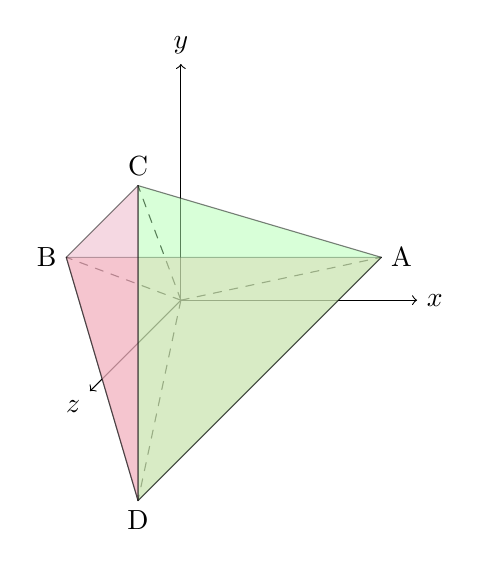
\begin{tikzpicture}[line join = round, line cap = round]

\pgfmathsetmacro{\factor}{1/sqrt(2)};
\coordinate [label=right:A] (A) at (2,0,-2*\factor);
\coordinate [label=left:B] (B) at (-2,0,-2*\factor);
\coordinate [label=above:C] (C) at (0,2,2*\factor);
\coordinate [label=below:D] (D) at (0,-2,2*\factor);

\draw[->] (0,0) -- (3,0,0) node[right] {$x$};
\draw[->] (0,0) -- (0,3,0) node[above] {$y$};
\draw[->] (0,0) -- (0,0,3) node[below left] {$z$};
\foreach \i in {A,B,C,D}
 \draw[dashed] (0,0)--(\i);
\draw[-, fill=red!30, opacity=.5] (A)--(D)--(B)--cycle;
\draw[-, fill=green!30, opacity=.5] (A) --(D)--(C)--cycle;
\draw[-, fill=purple!30, opacity=.5] (B)--(D)--(C)--cycle;
\end{tikzpicture}

\end{document}
